% ----------------------------------------------------------------------
% JSM Presentation 
% Author: Robert Clements  <clements@stat.ucla.edu>
% Date: 06/01/2010
% ----------------------------------------------------------------------

\documentclass[11pt]{beamer}

%%% To get handouts:
% \documentclass[11pt,containsverbatim,handout]{beamer}

% Load packages
\usepackage{graphicx}
\usepackage{amsfonts}
\usepackage{amsmath}
\usepackage{amssymb}
\usepackage{epstopdf}
\usepackage{listings}
\usepackage{fancybox}

%there are other themes to use, check online
\usetheme{Copenhagen}
%% include when making handouts
 % \usepackage{pgfpages}
 % \pgfpagesuselayout{4 on 1}[letterpaper,landscape,border shrink=5mm]



% Title
% Note: [short title]{long title}, [short author(s) name]{long author(s) name}
\title[Super-thinning]{Model Assessment for Space-time Point Processes Using Super-thinning}
%\subtitle{}
\author[RA Clements \and RP Schoenberg \and A Veen]{Robert Alan Clements\\ \and Rick Schoenberg\\ \and Alejandro Veen}
\date{\today}

% Presentation
% ----------------------
\begin{document}
% --------------------------------------------------- Title Frame --
\frame{ \titlepage }
% --------------------------------------------------- Intro

%----------------------Part----------------------

\part{Background}
\begin{frame}
  \partpage
\end{frame}

\section{Background}
\subsection{Spatial-temporal Point Processes}
\frame{
	\frametitle{\centerline{Point processes}}
	\begin{itemize}
   		\item random collections of points in some metric space 
  		 \item (locally) $\sigma$-finite: finitely many points within any bounded set
 		  \item simple: points at distinct locations and times
		  \item examples: earthquakes, wildfires, crime locations, etc. 
  	 \end{itemize}
  \begin{figure}
  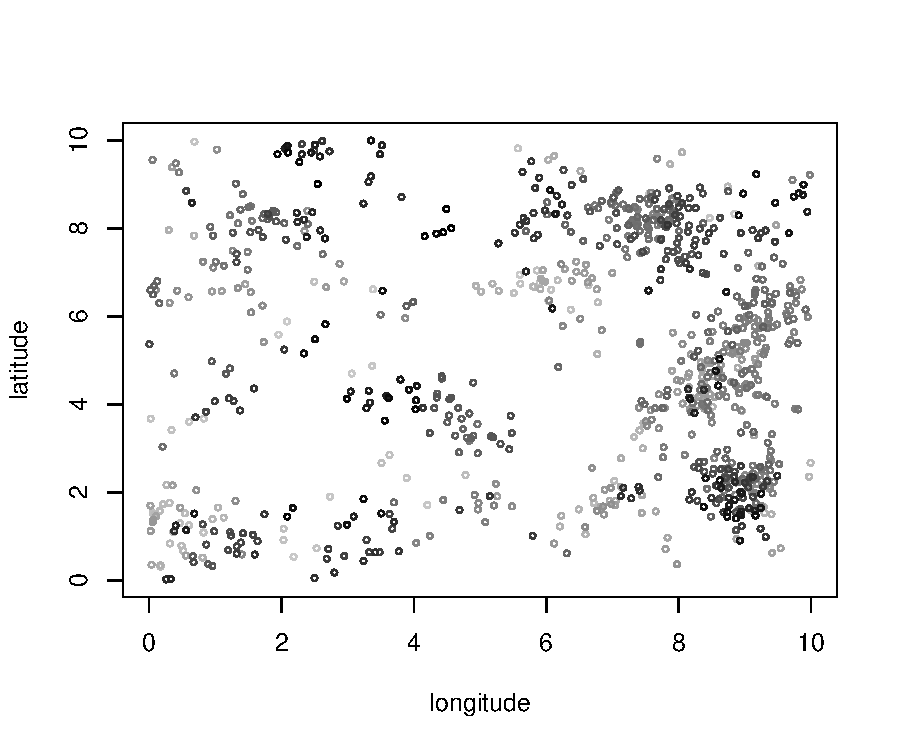
\includegraphics[scale=.40]{testfinal.pdf}
  \end{figure}
}
   
%\frame{
 % 	\frametitle{\centerline{Poisson processes}}
%	\begin{itemize}
%		\item for any set $B$, the number of points in $B$, $N(B)$, follows a Poisson distribution
%		\item no clustering, no inhibition
 % 		\item the homogeneous (stationary) Poisson process
 %  		\begin{itemize}
 % 			 \item completely spatially random
 % 			 \item any clustering is by chance
 % 		\end{itemize}
 %  		\item the inhomogeneous (non-stationary) Poisson process
 %  		\begin{itemize}
 %  			\item Poisson process with rate as a function of time (or space)
 %  		\end{itemize}
 % 	 \end{itemize}
%}


\frame{
  	\frametitle{\centerline{The conditional intensity}}
  	\begin{itemize}
  		\item the conditional intensity $\lambda(x,y,t)$ is defined as the frequency with which events are expected to occur in a space S around a specific point, time and mark (for marked point processes), conditional on the prior history $\mathcal{H}_{t}$ (Daley and Vere-Jones, 2003)
		\vskip1cm
  		\item $\lambda$ uniquely characterizes a simple point process 
  		\vskip1cm
  		\shadowbox{
  $\lim\limits_{\Delta x, \Delta y, \Delta t \downarrow 0}\frac{E[N\{(x,x+\Delta x)\times(y, y+\Delta y)\times(t, t+\Delta t)\}|\mathcal{H}_{t}]}{\Delta x \Delta y \Delta t}$
  }
  \end{itemize}
}

\frame{
	\frametitle{\centerline{Hawkes process}}
	\begin{itemize}
		\item useful for modeling earthquakes (Ogata 1988, 1998)
		\item cluster process
		\begin{itemize}
			\item {\color{purple}background points} (immigrants) trigger {\color{teal}offspring points} (1st generation descendants)
			\item {\color{teal}offspring points} trigger their own {\color{teal}offspring points} (2nd generation descendants)
		\end{itemize}
		\item modeled by \[\lambda(x, y, t) = {\color{purple}\mu(x, y, t)} + \sum_{\{i:t_{i}<t\}} {\color{teal}g(x-x_{i}, y-y_{i}, t-t_{i})}\]
	\end{itemize}

}

\frame{
	\frametitle{\centerline{Hawkes process}}
	 {\scriptsize \[\lambda(x, y, t) = 0.02 + \sum_{\{i:t_{i}<t\}} K_{0}\frac{\alpha \beta}{\pi}e^{-\alpha t - \beta(x^{2}+y^{2})}\]}
 \begin{figure}
  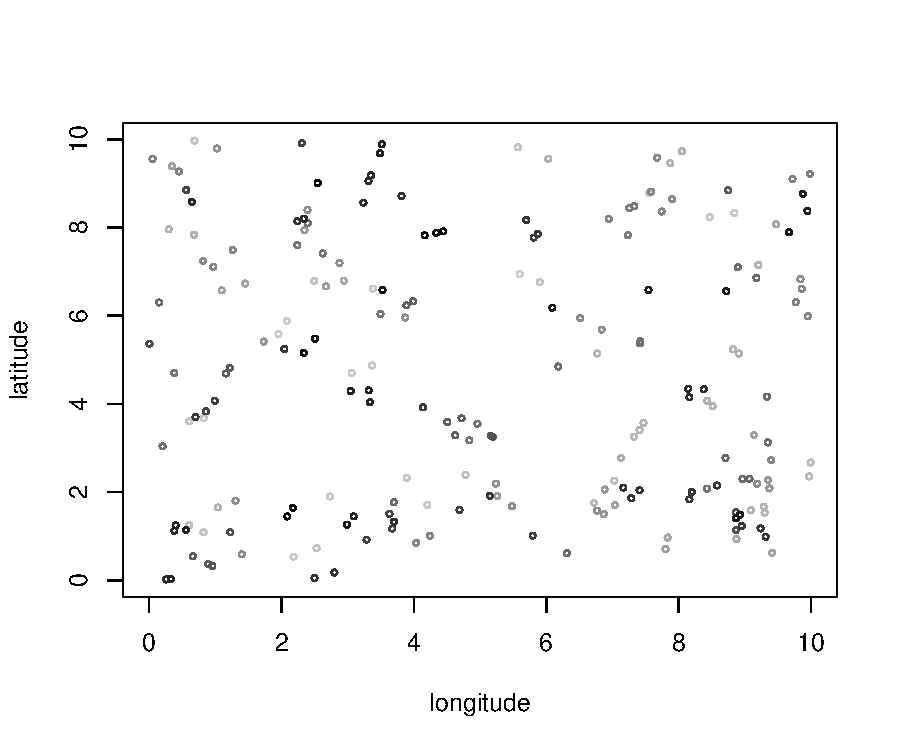
\includegraphics[scale=.40]{test1.pdf}
  \end{figure}
}

\frame{
	\frametitle{\centerline{Hawkes process}}
	 {\scriptsize \[\lambda(x, y, t) = 0.02 + \sum_{\{i:t_{i}<t\}} K_{0}\frac{\alpha \beta}{\pi}e^{-\alpha t - \beta(x^{2}+y^{2})}\]} 
	\begin{figure}
  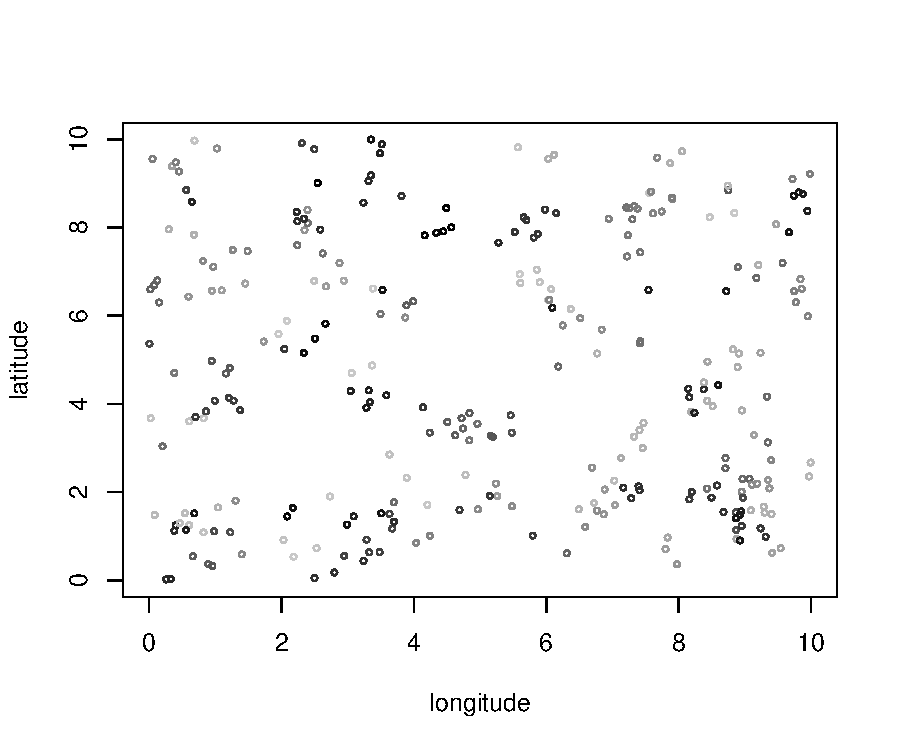
\includegraphics[scale=.40]{test2.pdf}
  \end{figure}
}

\frame{
	\frametitle{\centerline{Hawkes process}}
	{\scriptsize \[\lambda(x, y, t) = 0.02 + \sum_{\{i:t_{i}<t\}} K_{0}\frac{\alpha \beta}{\pi}e^{-\alpha t - \beta(x^{2}+y^{2})}\]}
	 \begin{figure}
  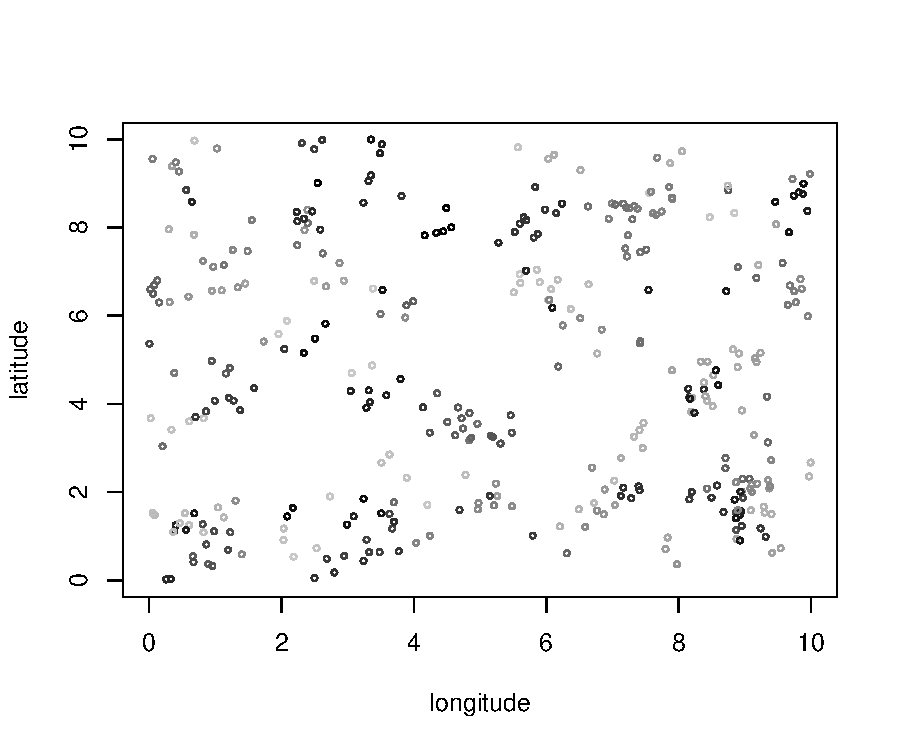
\includegraphics[scale=.40]{test3.pdf}
  \end{figure}
}

\frame{
	\frametitle{\centerline{Hawkes process}}
	{\scriptsize \[\lambda(x, y, t) = 0.02 + \sum_{\{i:t_{i}<t\}} K_{0}\frac{\alpha \beta}{\pi}e^{-\alpha t - \beta(x^{2}+y^{2})}\]}
	 \begin{figure}
  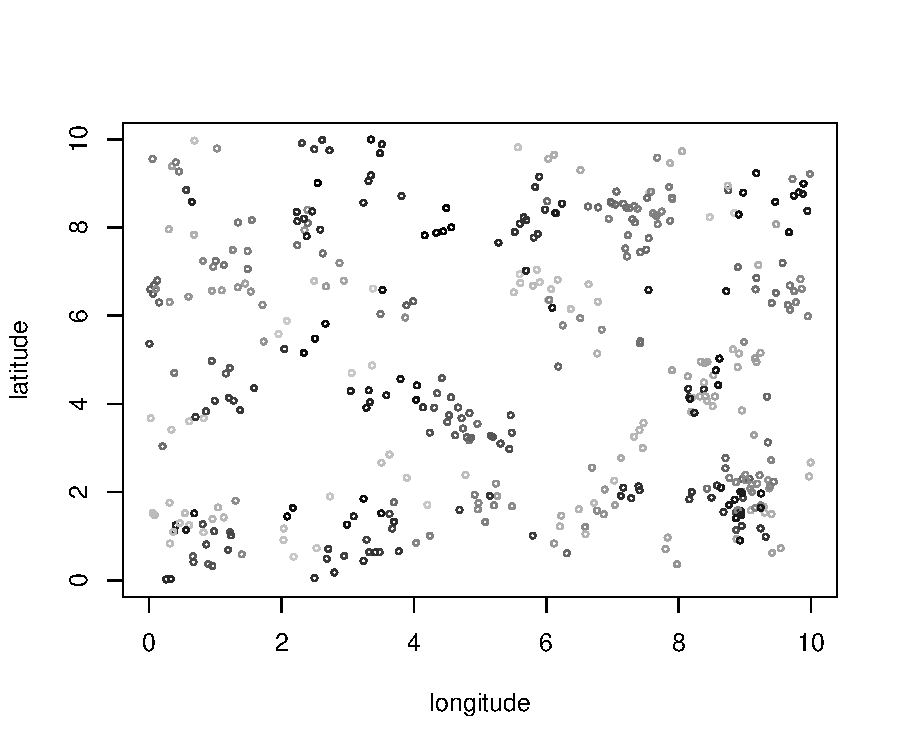
\includegraphics[scale=.40]{test4.pdf}
  \end{figure}
}

\frame{
	\frametitle{\centerline{Hawkes process}}
	{\scriptsize \[\lambda(x, y, t) = 0.02 + \sum_{\{i:t_{i}<t\}} K_{0}\frac{\alpha \beta}{\pi}e^{-\alpha t - \beta(x^{2}+y^{2})}\]}
	 \begin{figure}
  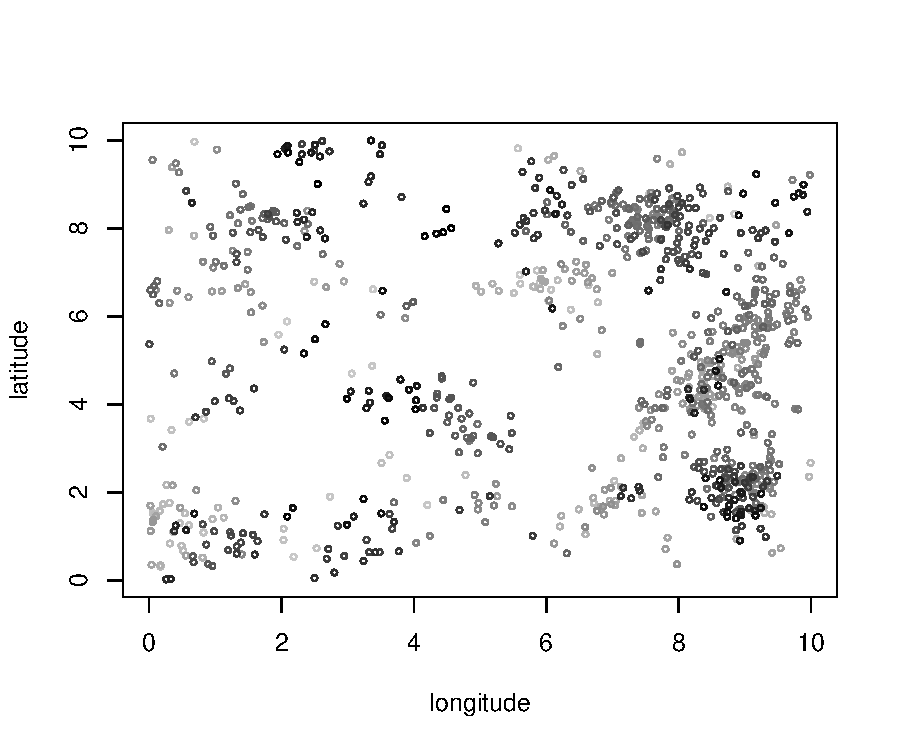
\includegraphics[scale=.40]{testfinal.pdf}
  \end{figure}
}

%----------------------Part----------------------
\part{Residual Analysis}
\begin{frame}
  \partpage
\end{frame}

\section{Residual Analysis}
\subsection{Superposition}
\begin{frame}
  	\frametitle{\centerline{{\color{yellow}Superposed} residuals}}
 	\begin{itemize}
		\item simulate points in $S$ with probability \[c - \hat{\lambda}(x, y, t) \mbox{ where } c = \mbox{sup}\{\hat{\lambda}(x, y, t)\} \mbox{ over } S\]
		\item essentially, superimpose a point process onto the existing point process, with conditional intensity \[\hat{\lambda}_{S}(x, y, t) = c - \hat{\lambda}(x, y, t) \]
		\item the result, called {\textit{superposed}} residuals, are homogeneous Poisson, with rate $c$, if fitted model is correct (Br\'emaud, 1981)
	\end{itemize}
\end{frame}

\frame{
  	\frametitle{\centerline{{\color{yellow}Superposed} residuals}}
	{\scriptsize \[\hat{\lambda}(x,y,t) = .02 + \sum_{\{i:t_{i}<t\}} K_{0}\frac{\alpha}{2\sigma^{2}\pi}exp\left\{-\alpha t - \frac{1}{2}\left(\frac{\sqrt{x^{2}+y^{2}}}{\sigma}\right)^{2}\right\}\]}
  	  \begin{figure}
 	 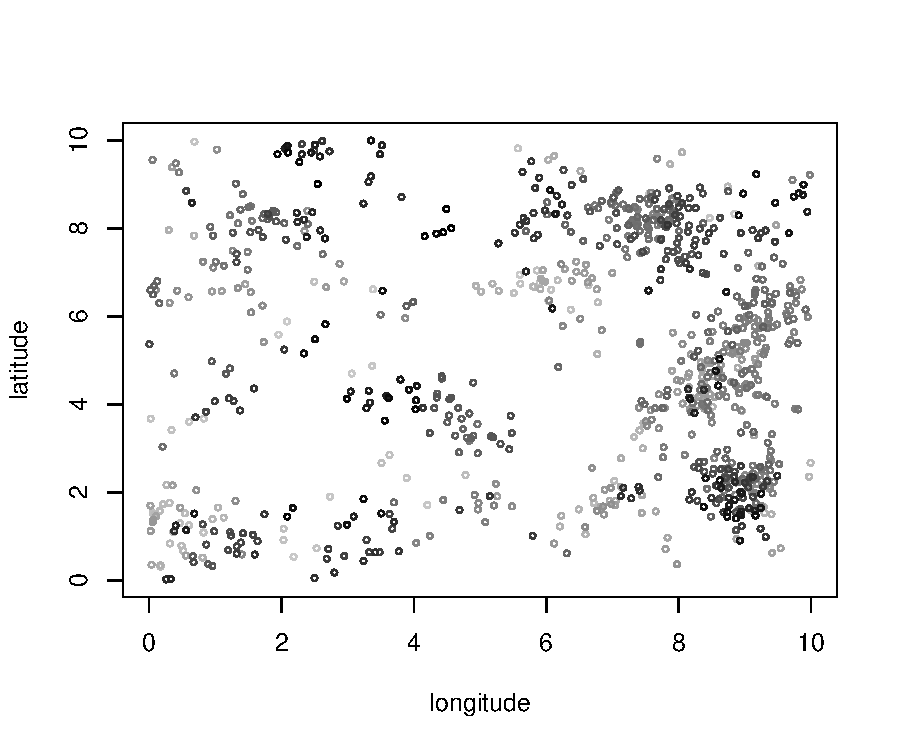
\includegraphics[scale=.40]{testfinal.pdf}
  	\end{figure}
}

\frame{
  	\frametitle{\centerline{{\color{yellow}Superposed} residuals}}
  	{\scriptsize \[\hat{\lambda}(x,y,t) = .02 + \sum_{\{i:t_{i}<t\}} K_{0}\frac{\alpha}{2\sigma^{2}\pi}exp\left\{-\alpha t - \frac{1}{2}\left(\frac{\sqrt{x^{2}+y^{2}}}{\sigma}\right)^{2}\right\}\]}
	 \begin{figure}
 	 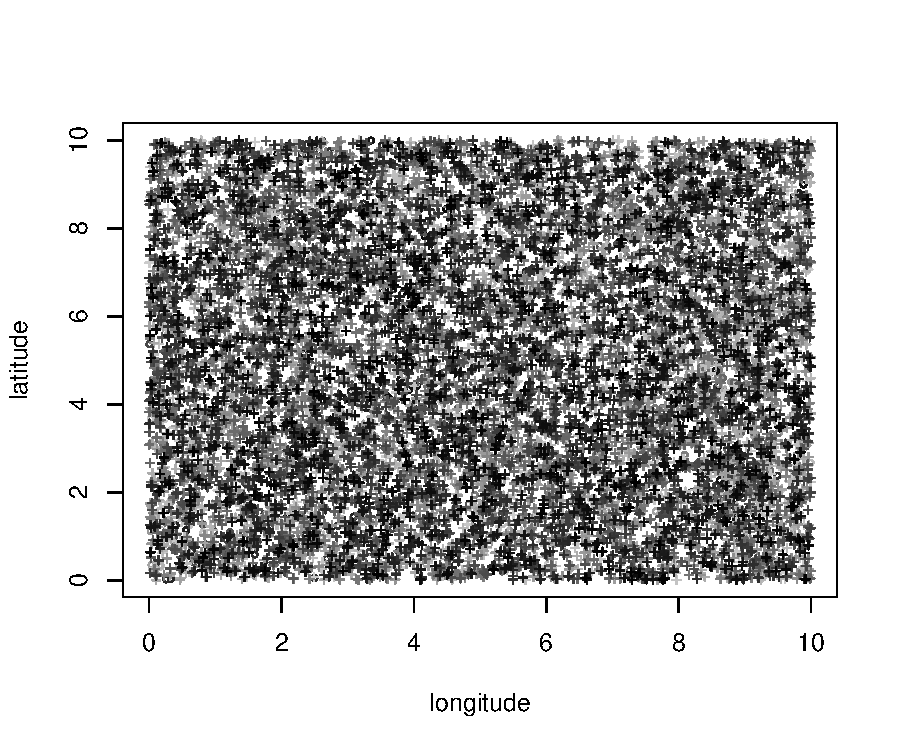
\includegraphics[scale=.40]{superplot.pdf}
  	\end{figure}
}

\subsection{Thinned Residuals}
\begin{frame}
	\frametitle{\centerline{{\color{green}Thinned} residuals}}
	\begin{itemize}
    		\item keep each observation in $S$ with probability \[\frac{b}{\hat{\lambda}(x_{i},y_{i}, t_{i})} \mbox{ where } b = \mbox{inf}\{\hat{\lambda}(x, y, t)\} \mbox{ over } S \]
    		\item remaining points, called {\textit{thinned}} residuals, are homogeneous Poisson, with rate $b$, if fitted model is correct (Schoenberg, 2003)
		\end{itemize}
\end{frame}

\frame{
  	\frametitle{\centerline{{\color{green}Thinned} residuals}}
	{\scriptsize \[\hat{\lambda}(x,y,t) = .02 + \sum_{\{i:t_{i}<t\}} K_{0}\frac{\alpha}{2\sigma^{2}\pi}exp\left\{-\alpha t - \frac{1}{2}\left(\frac{\sqrt{x^{2}+y^{2}}}{\sigma}\right)^{2}\right\}\]}
  	  \begin{figure}
 	 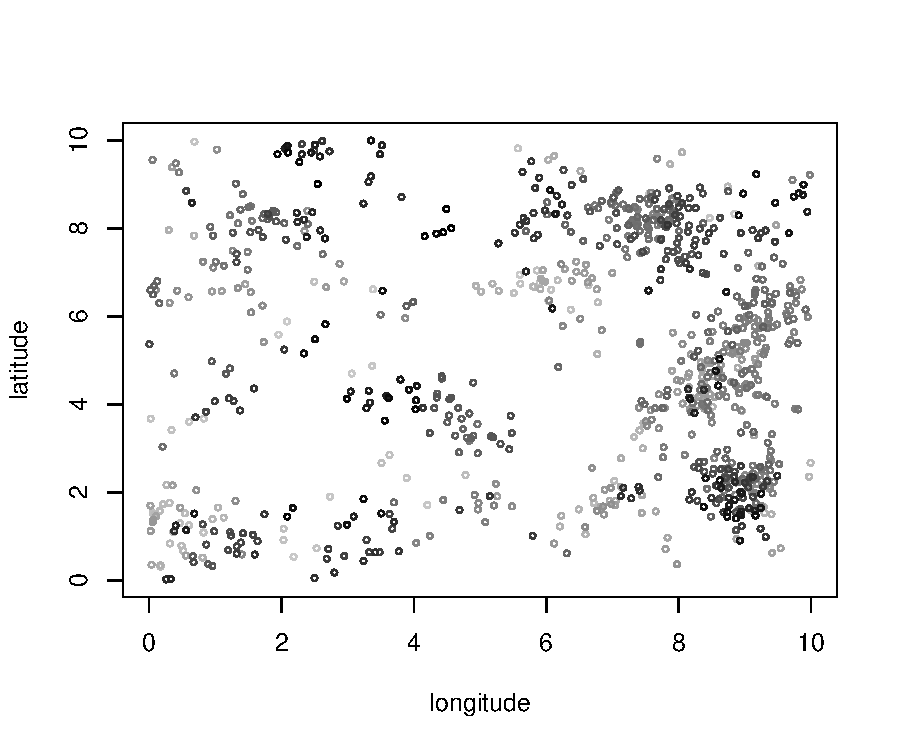
\includegraphics[scale=.40]{testfinal.pdf}
  	\end{figure}
}

\frame{
  	\frametitle{\centerline{{\color{green}Thinned} residuals}}
  	{\scriptsize \[\hat{\lambda}(x,y,t) = .02 + \sum_{\{i:t_{i}<t\}} K_{0}\frac{\alpha}{2\sigma^{2}\pi}exp\left\{-\alpha t - \frac{1}{2}\left(\frac{\sqrt{x^{2}+y^{2}}}{\sigma}\right)^{2}\right\}\]}
	 \begin{figure}
 	 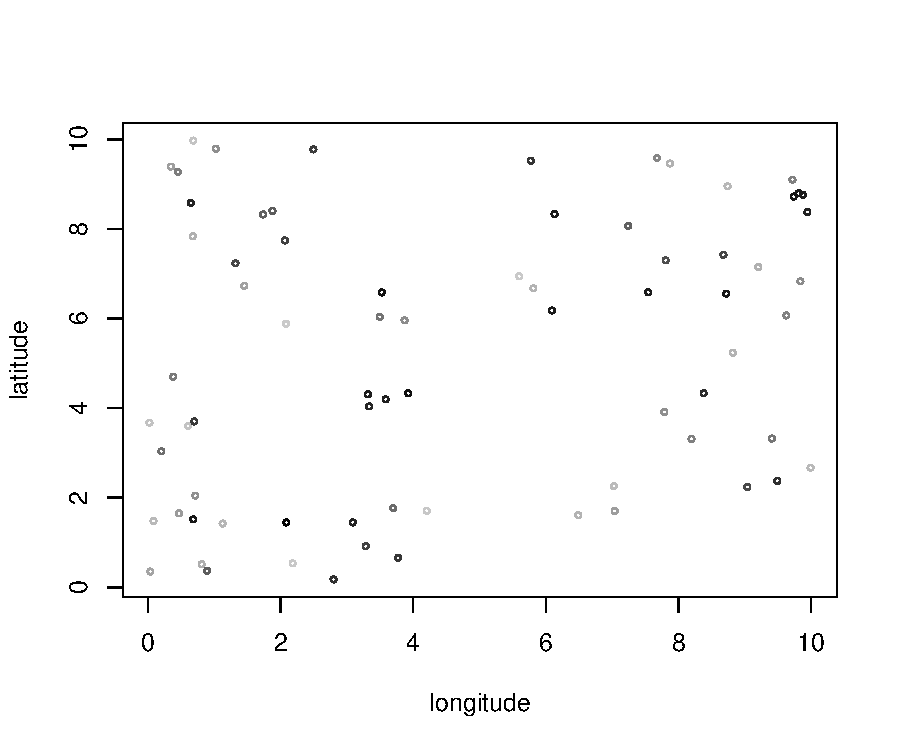
\includegraphics[scale=.40]{thinplot.pdf}
  	\end{figure}

}

\subsection{Super-thinned Residuals}
\begin{frame}
	\frametitle{\centerline{{\color{yellow}Super}-{\color{green}thinned} residuals}}
	\begin{itemize}
		\item thin points if $\hat{\lambda}(x_{i}, y_{i}, t_{i}) \geq k$
		\begin{itemize}
			\item keep each point with probability $\frac{k}{\hat{\lambda}(x_{i}, y_{i}, t_{i})}$
		\end{itemize}
		\vskip1cm
		\item simulate points if $\hat{\lambda}(x, y, t) < k$
		\begin{itemize}
			\item simulate points with probability $k - \hat{\lambda}(x, y, t)$
		\end{itemize}
		\vskip1cm
		\item the result, called \textit{super-thinned} residuals, is homogeneous Poisson, with rate $k$, if fitted model is correct
	\end{itemize}
\end{frame}

\frame{
  	\frametitle{\centerline{{\color{yellow}Super}-{\color{green}thinned} residuals}}
	{\scriptsize \[\hat{\lambda}(x,y,t) = .02 + \sum_{\{i:t_{i}<t\}} K_{0}\frac{\alpha}{2\sigma^{2}\pi}exp\left\{-\alpha t - \frac{1}{2}\left(\frac{\sqrt{x^{2}+y^{2}}}{\sigma}\right)^{2}\right\}\]}
  	 \begin{figure}
 	 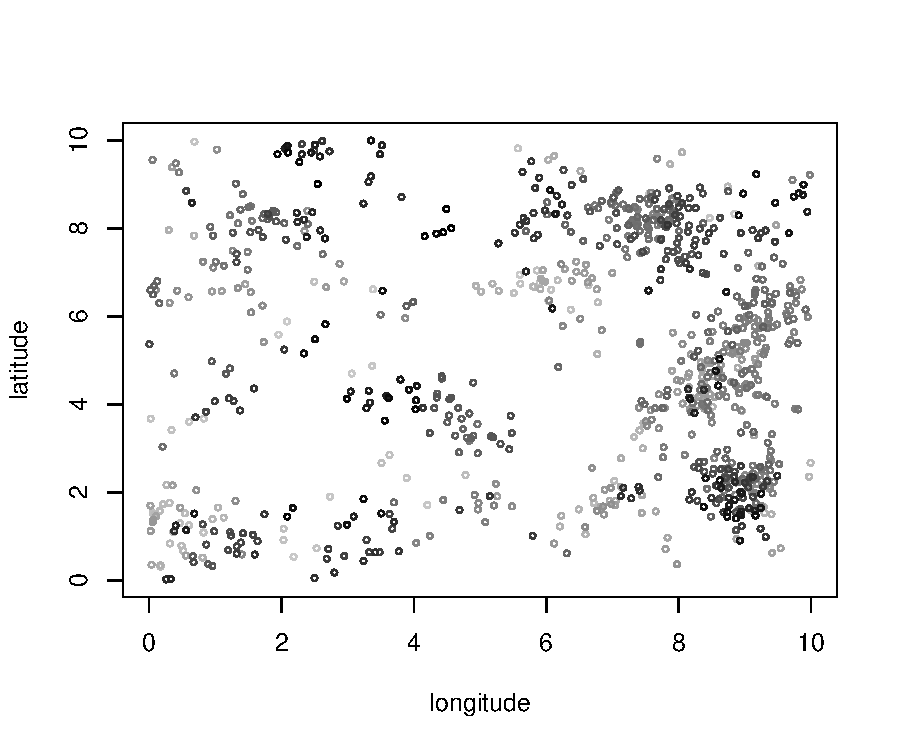
\includegraphics[scale=.40]{testfinal.pdf}
  	\end{figure}
}

\frame{
  	\frametitle{\centerline{{\color{yellow}Super}-{\color{green}thinned} residuals}}
  	\[k = \frac{250}{|S|} = 0.0833\]
	 \begin{figure}
 	 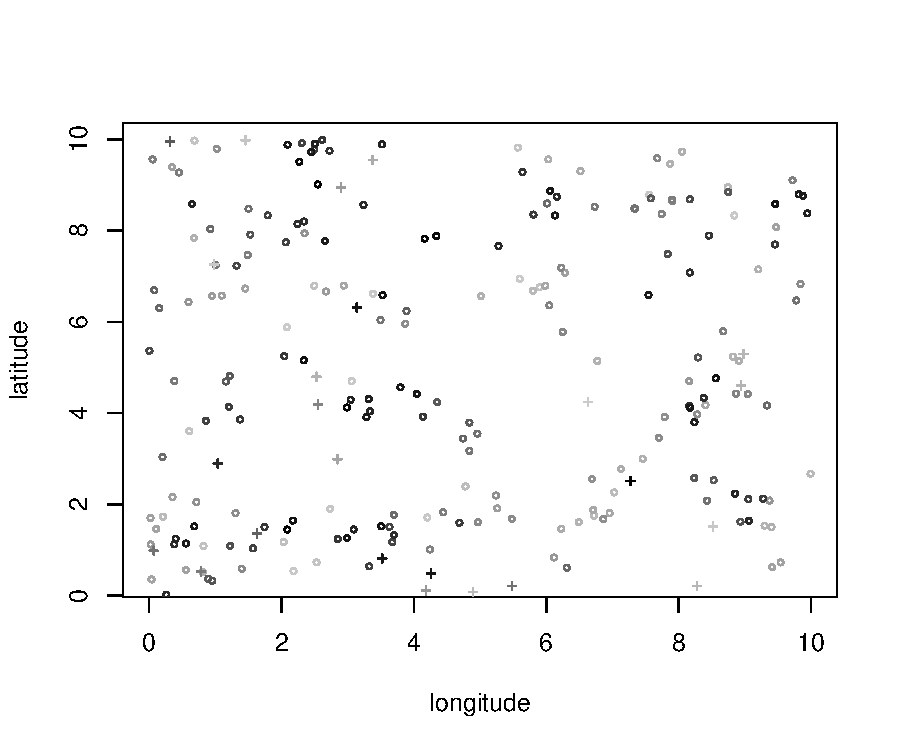
\includegraphics[scale=.40]{superthinplotk1.pdf}
  	\end{figure}
}

\frame{
  	\frametitle{\centerline{{\color{yellow}Super}-{\color{green}thinned} residuals}}
  	\begin{itemize}
		\item some choices of $k$ seem to be more powerful than others
   		\item how should we choose $k$?
		\item common sense choices:
		\begin{itemize}
			\item choose $k$ such that the same number of points are thinned and superposed (the mean of $\lambda$)
			\item choose $k$ such that the fewest number of points are thinned and superposed (the median of $\lambda$)
		\end{itemize}
  	\end{itemize}
}

%\frame{
 % 	\frametitle{\centerline{{\color{yellow}Super}-{\color{green}thinned} residuals}}
 % 	\[k = \frac{400}{|S|} = 0.133\]
%	 \begin{figure}
 %	 \includegraphics[scale=.40]{superthinplotk2.pdf}
  %	\end{figure}
%}

%\frame{
 % 	\frametitle{\centerline{{\color{yellow}Super}-{\color{green}thinned} residuals}}
 % 	\[k = \frac{600}{|S|} = 0.20\]
%	 \begin{figure}
 %	 \includegraphics[scale=.40]{superthinplotk3.pdf}
  %	\end{figure}
%}

\frame{
  	\frametitle{\centerline{{\color{yellow}Super}-{\color{green}thinned} residuals}}
  	\[k = \frac{889}{|S|} = 0.2963\]
	 \begin{figure}
 	 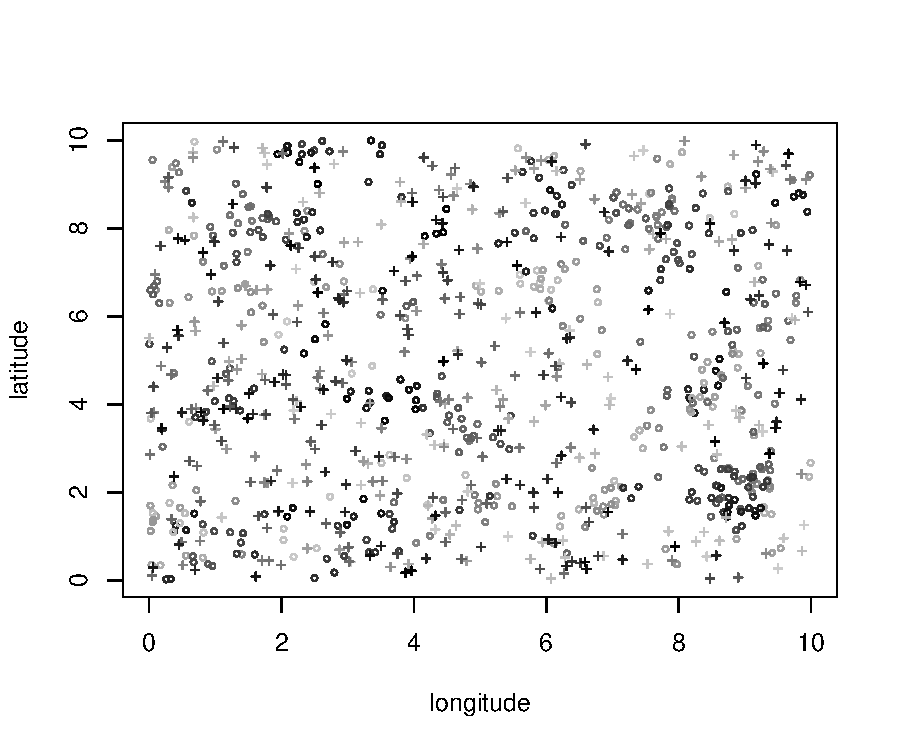
\includegraphics[scale=.40]{superthinplotk4.pdf}
  	\end{figure}
}

\section{Summary}
\frame{
 	\frametitle{\centerline{Summary}}
 	\begin{itemize}
 		\item superposition may result in too many points, which is difficult to interpret
 		\item thinning may result in too few points
 		\item super-thinning is a more powerful alternative due to the tuning parameter, $k$
		\item open question: which value of $k$ is most powerful?
 	\end{itemize}
}
%%%%%%%%%%%%%end of talk%%%%%%%%%%%%%%%%

\section{Contact}
\begin{frame}

\begin{center}
Thank you for attending!
\end{center} 
\vspace{1.5cm}
\begin{center}
Contact info:\\
Robert Clements\\
Department of Statistics, UCLA\\
clements@stat.ucla.edu
\end{center}

\end{frame}

\end{document}
%%%%%%%%%%%%%%%%%%%%%%%%%%%%%%%
%%%%%%%%%%%%%%%%%%%%%%%%%%%%%%%
%%%%%%%%%%%%%%%%%%%%%%%%%%%%%%%




